% vim:tw=72 sw=2 ft=tex
%         File: robosub.tex
% Date Created: 2016 Aug 08
%  Last Change: 2016 Aug 08
%     Compiler: pdflatex
%       Author: batumon
\documentclass[12pt,a4paper]{article}
\usepackage{amsmath, amssymb}
\usepackage[utf8]{inputenc}
\usepackage[T1]{fontenc}
\usepackage[english]{babel}
\usepackage[final]{graphicx}
\graphicspath{{./fig/}}

\begin{document}
\tableofcontents
\newpage

\section{Journey}
If one merely wishes to type in ordinary text, without
complicated mathematical formulae or special effects such
as font changes, then one merely has to type it in as it
is, leaving a completely blank line between successive
paragraphs.

You do not have to worry about paragraph indentation:
all paragraphs will be indented with the exception of
the first paragraph of a new section.

\begin{figure}[h]
      \centering
      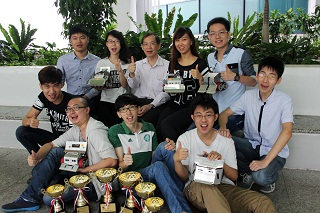
\includegraphics[scale=0.7]{jiaming}
      \caption{\label{fig:homofilter} An illustration of the quick brown fox \emph{jumping} over the lazy dog.}
\end{figure} 
\newpage

\section{Obstacles}
One must take care to distinguish between the `left quote'
and the `right quote' on the computer terminal.  Also, one
should use two `single quote' characters in succession if
one requires ``double quotes''.  One should never use the
(undirected) `double quote' character on the computer
terminal, since the computer is unable to tell whether it
is a `left quote' or a `right quote'.  One also has to
take care with dashes: a single dash is used for
hyphenation, whereas three dashes in succession are required
to produce a dash of the sort used for punctuation---such as
the one used in this sentence \cite{wang2005modular}.

\bibliography{robosub}
\bibliographystyle{ieeetr}
\end{document}
